%------------------------------------------------------------------------
% Chapter:  Build in defect models
%------------------------------------------------------------------------

\chapter{Build in defect models \label{mod}}

The following built in defect models modify the whole structure.
They offer extended defects that include modification of many
atoms throughout the whole crystal.  While such modifications
could be achieved as well by the user through extended use of the
FORTRAN interpreter, this would require extremely lengthy and
necessarily slow macros.  Defect models built in the source code
of the program on the other hand are calculated in much shorter
time.  The defect models were implemented with as many general
features as seemed necessary.  They use separate sub menus to
define the intended defect structure.

%------------------------------------------------------------------------

\section{Thermal displacements \label{mod-therm}}

The command {\tt therm} can be used to randomly displace all atoms
or rigid molecules of the crystal as to be expected by purely random
thermal disorder.  The direction of the displacement is distributed
with a uniform random spherical distribution.  The amplitude of the
displacement is distributed by a Gaussian distribution.  The mean of
the distribution is zero, its sigma is calculated from the isotropic
thermal coefficient, B, of each atom as:
%
\begin{equation}
    \langle u^{2} \rangle = \frac{B}{8 \pi^{2}}
    \label{therm-eq1}
\end{equation}
%
After the command {\tt therm} is executed, a summary of theoretical
and achieved displacement averages is displayed on the screen. An
example is shown below:
%

\begin{MacVerbatim}
   Thermal displacements summary :

                 Input               Achieved             Maximum displacement
   Atom        B   <u**2>     <ux**2> <uy**2> <uz**2>        x      y      z
   ---------------------------------------------------------------------------
   LA(1)     0.34  0.0043      0.0043  0.0043  0.0044     0.2299 0.2450 0.2487
   MN(2)     0.21  0.0027      0.0027  0.0027  0.0026     0.1980 0.1868 0.2184
   O(3)      0.50  0.0063      0.0061  0.0063  0.0064     0.2827 0.3518 0.3011
   O(4)      0.43  0.0054      0.0054  0.0055  0.0055     0.2745 0.3036 0.2855
\end{MacVerbatim}
%
The first column lists the name of the atom type followed by the B
and corresponding $\langle u^{2} \rangle$ value. The next three
columns show the achieved $\langle u_{i}^{2} \rangle$ values for
the x-, y- and z-direction. The last three columns give the
maximum displacements in the three directions that were
introduced. The values are given in \AA$^{2}$ and \AA. \par

The parameter {\tt mol} will displace rigid molecules according to
the B value of the atom at the origin of the molecule. Furthermore
the parameter {\tt 2d} allows to restrict the displacements to
directions with more than one unit cell extension of the crystal.
This might be used when working with 2-dimensional model crystals
where a displacement in the third direction is not wanted.

%------------------------------------------------------------------------

\section{Modulations \label{mod-wave}}

The given structure can be modulated using the {\tt wave} segment of
the program \Discus. Three different types of waves are
available, density waves modulating the occupation of sites within
the crystal, displacements waves modulating the position of atoms or
molecules and rotational waves which modulate the orientation of
molecules by rotating them around a user defined axis. First common
features shall be described followed by details about the different
wave types in separate sections. \par

\Discus offers three different wave functions $w({\bf r})$,
sinusoidal, square and saw tooth defined in equations
\ref{wave-eq1}, \ref{wave-eq2} and \ref{wave-eq3}, respectively. The
parameter $\delta$ for the box shaped wave functions determines its
asymmetry. The symmetric case is given by $\delta = 0.5$. The
computed value of $w({\bf r})$ modulates density, position or
orientation as a function of the position ${\bf r}$ within the
crystal depending on the wave type selected.
%
\begin{eqnarray}
    w({\bf r}) & = & A \cos (2\pi\left [
                    \frac{{\bf kr}}{\lambda}+\psi\right ]) + A_{0}
    \label{wave-eq1}  \\
    w({\bf r}) & = & \left \{
       \begin{array}{ll}
       A+A_{0} & \mbox{for $\frac{\delta}{2} \leq
                            \left | \frac{\bf kr}{\lambda}+
                                \frac{\psi}{360^\circ} \right | <
                            1 - \frac{\delta}{2}$}\\
       A_{0}   & \mbox{otherwise}\\
       \end{array} \right.
    \label{wave-eq2}  \\
    w({\bf r}) & = & A \left [\frac{{\bf kr}}{\lambda}+
                                  \frac{\psi}{360^\circ} \right ] + A_{0}
    \label{wave-eq3}
\end{eqnarray}
%
The following list describes the different properties common to all
wave types that can be defined by the user.
%
\begin{itemize}
    \item  {\it Wave vector ${\bf k}$:}
    The wave vector ${\bf k}$ defines the {\it traveling} direction of the wave.
    The vector is defined using the {\tt vect} command in multiples of the base
    vectors of the crystal, i.e.  in unit cell units.

    \item  {\it Wave length $\lambda$:}
    The wave length $\lambda$ of the modulation wave is entered using
    the {\tt len} command. Note that $\lambda$ must be given in \AA.

    \item  {\it Amplitude $A$:}
    The amplitude $A$ defines the upper limit of displacements (in \AA) or
    rotation angle (in degrees). In case of density waves the probability
    of replacing an atom or molecule oscillates between an upper and
    lower limit (see section \ref{mod-wave-dens}). The command to set the
    amplitude $A$ is {\tt amp}.

    \item  {\it Constant offset $A_{0}$:}
    A constant displacement or rotation angle can be added to all
    selected atoms or molecules using the command {\tt amp0}.

    \item  {\it Phase $\psi$:}
    The phase $\psi$ of the atom or molecule at (0,0,0) can be altered via the
    command {\tt phase}.
\end{itemize}
%
The argument $[{\bf kr} / \lambda +\psi / 360^\circ]$ of the wave
functions is limited to the range of -1 to 1 for the box and saw
tooth function and to a range of $\pm 2 \pi$ for the sinusoidal wave
function.  The origin of the vector ${\bf r}$ is the crystals
origin.  \Discus allows the user to select which of the atoms
in the crystal are to be modified by the wave function.

\subsection*{Density waves \label{mod-wave-dens}}

Displacement waves are selected using the {\tt dens} command.  A
density wave replaces an existing atom or molecule by another atom
or molecule type or alternatively removes the atom or molecule. The
direction of the density wave is along the wave vector. A lower and
upper probability $P_{low}$ and $P_{high}$ for replacing an atom or
molecule must be provided using the command {\tt plow} and {\tt
phigh}. The probability for the current atom or molecule to remain
in the structure oscillates between these two values. The
parameters $A$ and $A_{0}$ are calculated from these two
probabilities. In case of a sinusoidal wave the parameters $A$ and
$A_{0}$ are defined by:
%
\begin{eqnarray}
    A     & = & \frac{1}{2} ( P_{high} - P_{low})
    \nonumber \\
    A_{0} & = & \frac{1}{2} ( P_{high} + P_{low})
    \label{wave-eq4}
\end{eqnarray}
%
In case of a box or saw tooth shaped wave function, the parameters
$A$ and $A_{0}$ are determined by the following equations:
%
\begin{eqnarray}
    A     & = & P_{high} - P_{low}
    \nonumber \\
    A_{0} & = & P_{low}
    \label{wave-eq4b}
\end{eqnarray}
%
A random number is calculated every time an atom is encountered
that had been selected.  If this random number is less than
$w({\bf r})$, the amplitude calculated by the wave function, the
atom or molecule is retained as was, otherwise it is deleted or
replaced by another atom or molecule. Its position is not changed.

\subsection*{Displacement waves \label{mod-wave-disp}}

Displacement waves are selected using the {\tt trans} command.  For
displacement waves, the wave function $w({\bf r})$ determines the
displacement of an atom or molecule along a given direction of
oscillation. The command {\tt osci} defines the oscillation
direction in lattice units. \Discus allows any direction of
that vector relative to the propagation direction of the wave.  In
cases where propagation and oscillation vector are parallel, we
speak of longitudinal waves. In cases where propagation and
oscillation are normal to each other we speak of a transversal wave.
\par

The default displacement mode is set to acoustic, i.e.  all atoms
are displaced in the same direction.  An (admittedly crude) optical
mode will displace all atoms that are identified as negative ions in
the opposite direction to all others.  Negative ions are recognized
through their respective name, e.g. {\tt CL1-}. As a side effect, if
charged ions are used, the Fourier transform will use the
corresponding scattering curve.  If this is to be avoided, calculate
the desired wave twice, once with positive amplitude and once with
negative, while selecting the corresponding atoms.

\subsection*{Rotational waves \label{mod-wave-rot}}

Another feature of \Discus are rotational waves limited to be
used with molecules.  Obviously rotating an atom around itself makes
no sense. Rotational wave are selected with the {\tt rot} command
followed by parameters defining the rotation axis relative to the
molecules origin in lattice units.  The wave function $w({\bf r})$
then modulates the rotation angle ${\phi}$ around this axis.
Additionally an optional offset relative to the molecule origin for
the rotation axis can be specified by the {\tt rot} command.
%
\begin{figure}[!tbh]
   \centering
   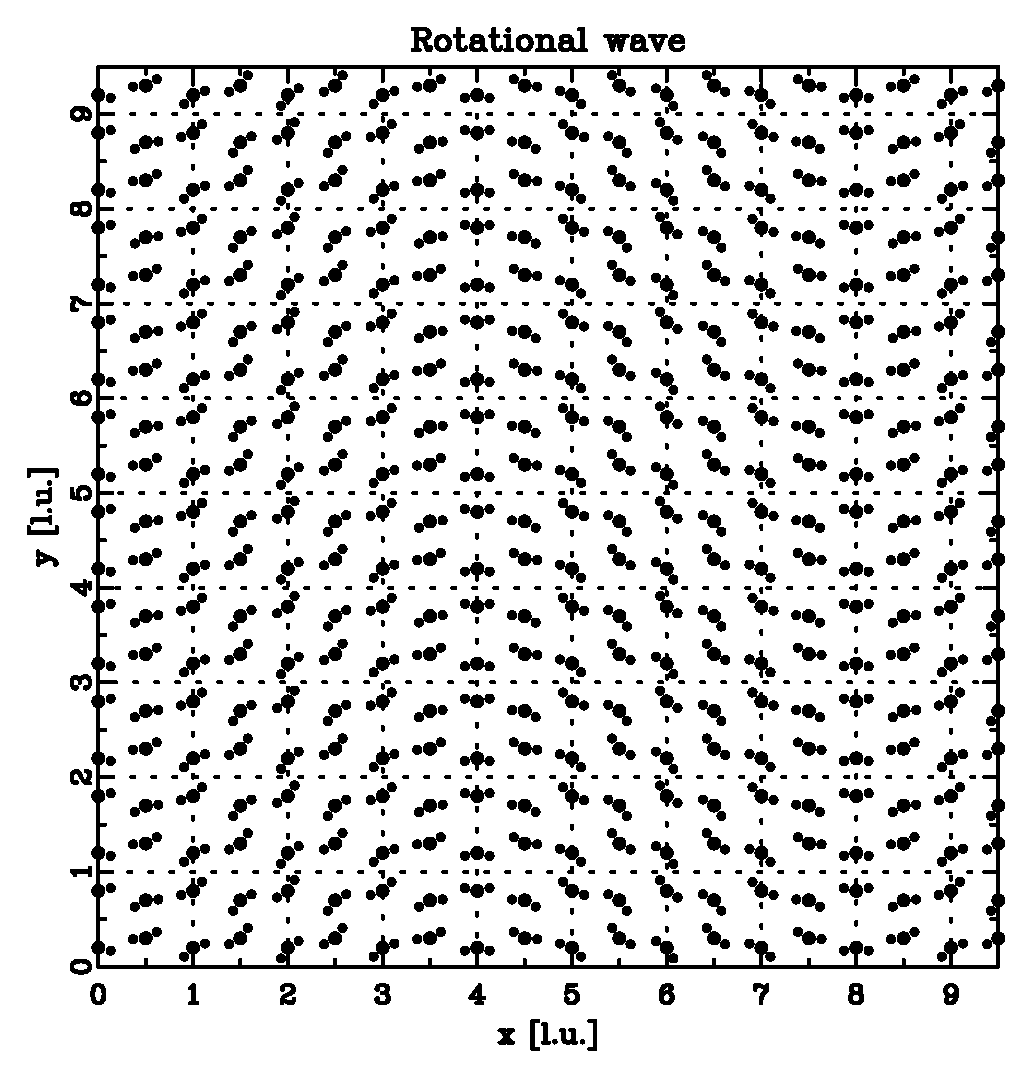
\includegraphics[scale=0.50, angle=0]{wave.3.eps}
   \caption{Example of a rotational wave}
   \label{wave-fig3}
\end{figure}
%
An example of such a rotational wave can be seen in figure
\ref{wave-fig3}. Here a cubic crystal with a size of 20x20x1 unit
cells (a = 10\AA) was used, each containing four $H_{2}O$ molecules.
The rotation axis is normal to the drawing plane, i.e. in
z-direction.  The wave vector is parallel to x and the wave length
$\lambda$ is eight unit cells (80 \AA).  The amplitude $A$ was set
to 45.0, i.e.  the rotation angle $\phi$ oscillates between $\pm 45$
degrees. \par

%------------------------------------------------------------------------

\section{Domains \label{mod-domain}}

The {\tt domain} module of \Discus has replaced the microdomain
module. A domain within \Discus is understood as a place holder
for an extended defect. This defect might be as small as an 
individual atom or be a region that extends over many unit cells.
 
Note, that in our book \citep{nedpro} we present examples using 
this domain module  and discuss domains at length. \par

As usual, the commands related to this modules are accessed after
entering the module via the command {\tt domain}. Let us look at a
simple example how to use this module:
%
\begin{MacVerbatim}
   1  domain
   2    rese
   3    mode   pseudo
   4    input  dom.cube.pseudo
   5    assign char,si,sphere
   6    assign fuzzy,si,0.5
   7    assign cont, si,dom.guest.cube.stru
   8    assign shape ,si,1,  1. , 0. , 0. ,  0.
   9    assign shape ,si,2,  0. , 1. , 0. ,  0.
  10    assign shape ,si,3,  0. , 0. , 1. ,  0.
  11    assign orient,si,1,  1. , 0. , 0. ,  0.
  12    assign orient,si,2,  0. , 1. , 0. ,  0.
  13    assign orient,si,3,  0. , 0. , 1. ,  0.
  14    show
  15    run
  16  exit
\end{MacVerbatim}
%
After resetting the module (line 2), mode {\tt pseudo} is selected.
In this mode, a \Discus structure file is used to define the
distribution of domains and each {\it pseudo atom} in this file is
later replaced by the corresponding domain. In our case, the atom Si
is replaced by the defined spherical domain (line 5). The boundary
is created by removing all atoms that are within 0.5\AA\ of the
domain (line 6). Next the domain dimension is define using the
matrix defined in lines 8--10. These values are in terms of unit
cells of the host structure. The second matrix (lines 11-13) defines
the orientation of the domain. Finally the settings are listed (line
14) and the domain is finally created (line 15). There is an
alternative extension of a structure file and the keyword {\tt
domain} allows to readily define the domain structure, its shape and
orientation (see \citet{nedpro}).
\par

%------------------------------------------------------------------------

\section{Stacking faults \label{mod-stack}}

All crystals whose structures can be described by layers are prone
to stacking faults.  A stacking fault is any defect that alters the
periodic sequence of layers.  These defects may be a wrong layer
inserted into the sequence, a change of the layer sequence or a
different translation between two subsequent layers.  These defects
may affect the whole crystal or a finite region if e.g. an
additional layer is present between an otherwise perfect sequence of
layers.  \Discus contains a tool to create layered crystal
structures and to introduce stacking faults into these crystals. The
crystals are formed in a two step procedure. First, the origin and
type of each layer is determined and second, the atoms corresponding
to each layer are introduced into the crystal.  The user can define
each layer type, the translation vectors between consecutive layers
and the correlation between neighboring layers. A new feature of the
stacking fault part of \Discus is the addition of rotational
disorder for the layer sequences. \par

The stacking fault sequence is defined by several parameters that
can be set in the {\tt stack} sub level of \discus:
%
\begin{itemize}
    \item  {\it Type of layers :}
    The positions of all atoms within a layer are read from a \Discus type
    structure file.  These layer files have to be created for each layer type
    involved beforehand using the various \Discus tools.

    \item  {\it Translations :}
    A translation vector between neighboring layers of each type must be
    provided.  Thus N different layer types result in a N*N matrix of
    translation vectors.  An example for translation vectors in a cubic face
    centered structure is given in table \ref{mod-stack-tab1}.

    \item  {\it Uncertainties for translation vectors:}
    In some materials small deviations in the translation vectors might occur.
    This behavior can be simulated in \Discus by setting a standard
    deviation $\sigma$ to each of the elements of the translation vector
    matrix.  \Discus will calculate the actual translation vector as sum
    of the 'ideal' vector plus a Gaussian distributed part defined by the value
    of $\sigma$.

    \item  {\it Correlations :}
    A correlation matrix is used to define the probabilities of two layer types
    to be nearest neighbors.  No further correlations are taken into account.
    To create correlations with {\it Reichweite} larger than 1, you can build 
    a one dimensional crystal of two or more atom types. The types and positions
    of these atoms can be interpreted as layer types and origins.

    \item  {\it Crystal shape :}
    The resulting crystal can be generated using two different modes: First,
    the crystal continuously grows in one direction as given by the translation
    vector(s).  Secondly one or two coordinates can be constrained to a finite
    range, which results in a zig-zag shaped crystal.  If any of the parameters
    is not equal to zero, the corresponding coordinate of the origin is taken
    modulo this parameter.  Note, that \Discus does not check whether the
    modulo vectors are translation vectors of the current space group.
\end{itemize}
%
\begin{table}[!tbh]
\centering
\begin{tabular}{|c|c|c|}
  \hline
  {\bf Layer type A} & {\bf Layer type B} & {\bf Translation vector} \\
  \hline\hline
  A & A & $(1, 1, 1)$ \\
  A & B & $\frac{1}{2} (1,1,0)$\\
  A & C & $\frac{1}{2} (1,0,1)$\\
  B & A & $\frac{1}{2} (\overline{1},\overline{1},0)$\\
  B & B & $(1, 1, 1)$\\
  B & C & $\frac{1}{2} (0,1,1)$\\
  C & A & $\frac{1}{2} (\overline{1},0,\overline{1})$\\
  C & B & $\frac{1}{2} (0,\overline{1},\overline{1})$\\
  C & C & $(1, 1, 1)$\\
  \hline
\end{tabular}
\caption{\label{mod-stack-tab1}Translation vectors for stacking
         faults in a cubic face centered structure}
\end{table}
%
The command {\tt create} in the {\tt stack} segment of \Discus
creates the list of layer origins and {\tt run} actually generates
the corresponding crystal by decorating the origins with the
individual layer types.  In order to speed up the calculation of the
Fourier transform, rather than using the resulting complete
structure, the scattering intensity is calculated in the following
way.  The scattering density $\rho ({\bf r})$ of a layered structure
can be expressed as the scattering density of the individual layer
types convoluted with the layer origin distribution.
%
\begin{equation}
    \rho({\bf r}) = \sum_{i=1}^{nl} \left \{ \sum_{j=1}^{no}
                    o_{ij} ({\bf r}) \right \} \star l_{i} ({\bf r})
    \label{mod-stack-eq1}
\end{equation}
%
The outer sum runs over all $nl$ layer types and the inner sum
runs over all origins $o_{ij}$ of layer type $i$.  The variable
$l_{i}$ is the scattering density of layer type $i$.  Using the
convolution theorem, the Fourier transform of this expression
becomes
%
\begin{equation}
    {\cal F} \left \{ \rho({\bf r}) \right \} =
        \sum_{i=1}^{nl}
              {\cal F} \left \{ \sum_{j=1}^{no} o_{ij} ({\bf r}) \right \}
        \cdot {\cal F} \{ l_{i} ({\bf r}) \}
    \label{mod-stack-eq2}
\end{equation}
%
Here ${\cal F}$ denotes the Fourier transform.  This procedure not
only speeds up the calculation but it also allows the usage of much
larger crystal sizes since the actual structure does not have to be
created in order to calculate the Fourier transform.
\par

%------------------------------------------------------------------------

\section{Surfaces \label{mod-surface}}

An initial model crystal will be a block of IxJxK unit cells. This shape
is ideal to avoid finite size effects when you want to calculate diffuse
scattering for an infinite large crystal. Nanoparticles or domains are
of course explicitly finite objects, whose shape you might want to 
control. \Discus offers the {\tt surface menu} to shape the crystal into
a finite sized object. The menu replaces the {\tt boundary} command that
is still available for backward compatibility.

Within the {\tt surface} menu, the {\tt boundary} command allows you to
shape the crystal by any combination of:\\
\begin{itemize}
\item an individual lattice plane {\tt HKL}
\item a form, i.e. a set of symmetrically equivalent lattice planes {\tt HKL}
\item a spherical surface
\item a triaxial ellipsoidal surface
\item a cylindrical surface
\end{itemize}

A plane will remove all atoms to one side of this plane:

\begin{MacVerbatim}
boundary hkl, 1, 1, -1, 15.0, inside
\end{MacVerbatim}

In this example a 11$\overline{1}$ plane is placed at 15.0\AA from the 
origin. All
atoms remain that are inside the boundary plane i.e. at the same side 
of the plane as is the origin 0.0, 0.0, 0.0. As a plane extends to 
infinity parallel to its surface, \Discus cannot create an object with
an indented surface using individual planes. 
Such an object can be build using a {\\tt form}, {\\tt sphere}, 
{\\tt ellipsoid} or {\\tt cylinder}.

A complete form of symmetrically equivalent faces can be created via:

\begin{MacVerbatim}
boundary form, 1, 1,  1, 15.0, inside
\end{MacVerbatim}

This will create an object that is limited by the complete set of
all symmetrically equivalent \{111\} faces. Keep in mind that this
set of faces will depend on the point group symmetry of your crystal!

A spherical object with radius R is created by the command:

\begin{MacVerbatim}
boundary sphere, 35.0, inside
\end{MacVerbatim}

A triaxial ellipsoid with diameters DX=20, DY=30, DZ=40 \AA\  is 
created by the command:

\begin{MacVerbatim}
boundary ellipsoid, 20, 30,40, inside
\end{MacVerbatim}

Admittedly it is a bit of an inconsistency that the "ellipsoidal" surface 
takes diameters instead of radii. Independent of the crystal system,
the three axes of the ellipsoid are always orthogonal to each other. 
The ellipsoid is oriented in a standard fashion. This orientation
is chosen such that the ellipsoid "Y"-axis is parallel to the 
crystallographic b-axis, the "Z" axis parallel to the c$*$ axis
and the "X" axis  forms a right handed orthogonal system. Table
\ref{mod-surf-tab1} lists the resulting orientations for the seven crystal systems:

\begin{table}[!tbh]
\centering
\begin{tabular}{|c|r|c|l|}
  \hline
  {\bf system} & {\bf X-axis} & {\bf Y-axis } & {\bf Z-axis} \\
  \hline\hline
  cubic        & {$\vec{a}$} = [100]                   & {$\vec{b}$} = [010]& {$\vec{c}$} = [001] \\
  hexagonal    & {$\vec{a^{*}}$} = [210]               & {$\vec{b}$} = [010]& {$\vec{c}$} = [001] \\
  trigonal     & {$\vec{a^{*}}$} = [210]               & {$\vec{b}$} = [010]& {$\vec{c}$} = [001] \\
  rhombohedral & {$\vec{b}\otimes\vec{c^{*}}$}         & {$\vec{b}$} = [010]& {$\vec{c^{*}}$}     \\
  tetragonal   & {$\vec{a}$} = [100]                   & {$\vec{b}$} = [010]& {$\vec{c}$} = [001] \\
  orthorhombic & {$\vec{a}$} = [100]                   & {$\vec{b}$} = [010]& {$\vec{c}$} = [001] \\
  monoclinic   & {$\vec{b}\otimes\vec{c^{*}}$} = [100] & {$\vec{b}$} = [010]& {$\vec{c^{*}}$}     \\
  triclinic    & {$\vec{b}\otimes\vec{c^{*}}$} = [100] & {$\vec{b}$} = [010]& {$\vec{c^{*}}$}     \\
  \hline
\end{tabular}
\caption{\label{mod-surf-tab1}Orientation of an ellipsoidal 
surface for the seven crystal systems.}
\end{table}

If the last parameter on the {\tt boundary} command is {\tt outside},
all those atoms are retained that are on the outside of the given
surface. For a single plane, only those atoms remain, that are on the 
outside of the surface. For the closed shapes {\tt form}, 
{\tt sphere}, {\tt ellipsoid}, {\tt cylinder} a cavity inside your
crystal will be the result. Keep in mind, that the {\tt form} will
not necessarily result in a true closed shape. Whether a closed
shape results depends on the actual Miller indices and the point 
group.


In order to create closed interior hollow spaces in low-symmetry 
structures, the shapes: {\tt sphere}, {\tt ellipsoid}, {\tt cylinder}
can be used in any crystal system. If the shape shall consist 
of flat surfaces you will likely need a combination of several
symmetrically non-equivalent faces to generate a closed shape.
\Discus provides optional parameters to the {\tt boundary command}
 for this  purpose:

\begin{MacVerbatim}
boundary  form, 1, 0,  1, 15.0,outside, accum:init, exec:hold
boundary  form, 1, 0, -1, 15.0,outside, accum:add , exec:hold
boundary  hkl , 0, 1,  0, 15.0,outside, accum:add , exec:hold
boundary  hkl , 0,-1,  0, 15.0,outside, accum:add , exec:run
\end{MacVerbatim}

The "accum:init" indicates to \Discus to initialize a list of
faces/forms. The actual cut is put on hold via the 
"exec:hold" statement. the next two commands add a further face
to the collection, while still keeping the execution on hold. 
The third statement finally adds the last face to make a 
completely closed shape in point group P2. As this is the final 
faces, the execution is performed via the "exec:run" parameter.

To shape an convex object, these two optional parameters are 
not needed, as each face may cut away the atoms independently.
For that reason, the two parameters default to
"accum:init" and "exec:run". 

Three further optional parameters allow you to place the center of the 
shape at an arbitrary point. These parameters take the style:

\begin{MacVerbatim}
boundary form, 1, 1,  1, 15.0, inside, centx:1.0, centy:2.0, centz:3.0
\end{MacVerbatim}

The colon ":" indicates that this is an optional parameter. The
value after the colon defines the respective position of the 
center along the three crystallographic axes. All values default
to zero.


%------------------------------------------------------------------------

\section{Decorating Surfaces \label{mod-deco}}

The {\tt decoration} menu within \Discus can be used to decorate
a surface with a group of additional atoms. The steps involved in such
a decoration process are two fold:
\begin{itemize}
\item Shape a crystal into the desired form via the {\tt surface} menu
\item Place one or several ligand molecules onto the surface
\end{itemize}

A common set of command to achieve this would be:
\begin{MacVerbatim}
 1  read
 2     cell structure.cell, 20, 20, 20
 3  surface
 4     boundary form, 1,0,0, lat[1]*4.5, keep:inside
 5  exit
 6  #
 7  decorate
 8     reset
 9     add example, normal
10     set example, ligand, ligand.stru, 0.015
11     set example, bond,   au, 1, 2.42
12     set example, axis, auto
13     set example, form,  1, 0, 0
14     show
15     run
16  exit
\end{MacVerbatim}

After the shaping of the crystal into a cube (here assuming a cubic 
structure in "structure.cell") \Discus enters the {\tt decorate} menu
in line 7. Once the mode is reset to ensure clean starting conditions,
a new decoration mode is {\tt added} in line 9. The string "example"
serves as a name for further references. The bonding style for this
decoration scheme is set to {\tt normal}. This will place the ligand
molecule with a single bond onto the surface and align the molecule
normal to the local surface. \Discus currently offers six bonding
schemes that are detailed further down. In line 10 we specify the
source of the decorating molecule as the file {\tt ligand.stru}. 
The molecule shall be placed onto the surface at a (rough) density of 
0.015 molecules per \AA$^2$. Line 11 specifies that a 
single bond between surface "Au" atoms and the first atom in 
ligand.stru should be build at a bond distance of 2.42\AA. \Discus is 
instructed in line 12 to align the molecule axis automatically.
Finally in line 13 the decoration is limited to surfaces that 
belong to the form \{100\} of the current crystal system. The 
standard {\tt show} and {\tt run} commands complete the action.

After this quick run through a more detailed explanation will follow. 
\Discus
will place the molecule contained in the file specified on the
{\tt ligand} instruction onto the surface of the particles. Prior
to this placement process, the particle must have been shaped via the 
{\tt surface} menu as \Discus relies on the surface property that is
generated in the {\tt surface} menu. Once you have chosen surface 
atoms onto which the guest molecules shall be placed, \Discus will
internally select these surface atoms and arrange these as evenly as 
possible on the surface. This distribution process attempts to
avoid overlap between the individual guest molecules. Admittedly 
this will not always be perfect, especially for a high surface 
density. If necessary use a lower density or use the {\tt mmc} 
menu to twist the guest molecules in order to avoid an overlap.

Currently \Discus offers six different bonding schemes for the 
nanoparticle decoration:
\begin{itemize}
\item {\tt normal} The molecule is placed with a single bond onto the
      surface. This bond is oriented normally to the local surface
      on top of the surface atom.
      Either automatically or via the pair of atoms provided via the
      {\tt axis} keyword, \Discus aligns the molecule itself normal
      the the surface as well.
\item {\tt bridge} The molecule is placed with two bonds onto the
      surface, midway between the two surface atoms. Both bonds 
      may have different lengths and a triangle results. The 
      two atoms within the surface and one atom within the ligand
      molecule form this triangle.
      The plane of this triangle is placed parallel to the local 
      surface normal.
      The remainder of the molecule is 
      aligned as in the {\tt normal} mode.
\item {\tt double} The molecule is placed with two bonds onto the
      surface. In contrast to the {\tt bridge} mode, two separate
      atoms from the ligand form respective bonds to two separate 
      surface atoms. Since the two bond may have different lengths, 
      the four atoms form a general quadrilateral. \Discus attempts
      to place the vector between the two molecule atoms parallel
      The plane of this quadrilateral is placed parallel to the local 
      surface normal.
      to the vector between the two surface atoms.
      The remainder of the molecule is 
      aligned as in the {\tt normal} mode.
\item {\tt multi} The molecule is placed with bonds between two
      molecule atoms to surface atoms. The first molecule atom
      builds two or more bonds of equal length to the corresponding
      number of surface atoms. The second molecule atoms forms a
      further single bond to a surface atom. The first atom is thus 
      in a generalized bridge position atop of the surface atoms. 
      If the surface group consists of four or more atoms, it will
      usually be impossible to obtain equal distances between the 
      molecule atom and all surface atoms. \Discus attempts to 
      place the atoms with as similar bonds as possible. Once the
      first molecule atom is placed, \Discus rotates the molecule
      to place the second molecule atoms into a position such 
      that it forms a single bond of specified length.
      The remainder of the molecule is 
      aligned as in the {\tt normal} mode.
\item {\tt acceptor} This mode serves to build a hydrogen bond 
      between a surface acceptor and a ligand molecule. 
      The user can specify the distance between the 
      surface acceptor atom and the "Hydrogen" atom in the molecule.
      This distance should of course be around 1.9\AA. This
      Hydrogen bond is placed normally to the local surface. \Discus 
      does not check if the atom in the molecule is actually a 
      Hydrogen atom, this responsibility is left to the user.
      As default \Discus rotates the molecule to achieve a 170$^\circ$
      bond angle in the Hydrogen atom.
      The remainder of the molecule is 
      aligned as in the {\tt normal} mode. In addition, the molecule
      is rotated by a random angle around the hydrogen bond.
\item {\tt donor} This counterpart to the {\tt acceptor} model 
      places the first molecule atom at the user specified hydrogen
      bond distance to the surface atom. Again, the distance should 
      be in the range of 1.9\AA\  and the surface atom should be a 
      hydrogen bond. The molecule atom is placed such that the 
      bond angle in the surface Hydrogen atom is by default
      170$^\circ$.
      The remainder of the molecule is 
      aligned as in the {\tt normal} mode. In addition, the molecule
      is rotated by a random angle around the covalent bond between 
      the surface hydrogen atom and its closest surface neighbor.
\end{itemize}

For each of these bonding schemes the user specifies the source of
the molecule. \Discus expects a standard structure file format as 
source. If your molecule resides in a {\tt CIF} file, please 
import this into the \Discus format first. The unit cell parameters
of the molecule do not have to be identical to those of the host
structure. \Discus will transform the coordinates internally.

For the bonding schemes {\tt acceptor} and {\tt donor} the 
hydrogen bond angle in the Hydrogen atoms defaults to 170$^\circ$.
To modify this angle \Discus provides the optional parameter
{\tt angle:value} to the {\tt set bond} command. 

\Discus will place the guest molecules at the user specified density 
(in molecules per square \AA ngstroem) onto the surface. This density
is roughly estimates using the number of surface atoms and assigning a
fixed area of 11\AA$^2$ to each surface atom. 

Depending on the bond scheme \Discus is left with freedom to align the complete
molecule. The schemes fix the position of the bonded molecule atoms only.
The remainder of the molecule is aligned roughly normal to the surface.
The user can specify a pair of atoms within the molecule or let \Discus
find the non-bonded molecule atom at furthest distance to the first
bonded molecule atom. Within the degrees of freedom of the bond scheme
the molecule is rotated to align the vector defined by these two atoms 
as close to the local surface normal as possible. For the {\tt normal}
, {\tt bridge} and {\tt donor} mode \Discus can freely rotated the 
molecule to achieve 
this orientation. For the {\tt double} and {\tt multiple} mode the 
molecule will be rotated around the vector between the two bonded molecule
atoms. As a result the molecule axis will be in the plane defined by the
surface atoms and the two bonded molecule atoms. This plane itself
is parallel to the surface normal. The molecule axis will be in this
plane but may still form an angle to the surface normal. For the
{\tt acceptor} mode, \Discus can rotate the molecule around the
Hydrogen-donor bond to align the molecule axis as close as possible to
the surface normal.

As default \Discus will place the guest molecule onto any surface atom type 
that occurs in any bond assignment. The user has the option to restrict
the placement onto an individual hkl plane or onto a form of symmetrically
equivalent planes. Thus, if you shaped the crystal into a polyhedron of
say the \{100\} and \{111\} faces, you have the option to restrict the 
placement onto either of the faces or forms.

When you use the {\tt boundary} command within the {\tt surface} menu to
shape the original crystal, \Discus will assign a surface property to 
those atoms that are close to the surface. Within the {\tt decorate} menu
\Discus uses this surface property to select atoms onto which a guest 
molecule can be placed. Thus it is mandatory to shape the crystal prior 
to any decoration. You may desire to build an initial crystal and to assign 
an external surface without actually removing any atoms. This might be
the case when you read a previously created structure that you want 
to decorate in a second step. In this case, you need to still "cut" 
the surface. In order not to remove any atoms, simply choose surfaces
parallel to the present surfaces and place these new surfaces just a little
bit outside the present surfaces. In combination with the 
{\tt set distance} command in the {\tt surface} menu atoms close to these
new surfaces will be flagged as surface atoms and can be used in the
decoration mode.

The atoms in the guest molecule receive a "Ligand" and a "Molecule" 
property, and these properties can be used for further manipulations.
The atoms do not automatically receive a surface property.
Currently \Discus does not try to decide which of the guest atoms are
at the "outside" in order to assign a correct surface property. It
appears the the molecule shape is too impredictable to do so fully
automatically. (\Discus may try to learn this in the future...)

The user can, however, assist by specifying guest molecule atoms 
that shall inherit the surface properties of the surface atom.
Use the command:

\begin{MacVerbatim}
set example, surface, atom_no
\end{MacVerbatim}
With this command, the listed atoms of the ligand molecule will 
receive the same surface properties as the original surface atom.
This will be useful, if you want to place a second layer of decorating 
molecules onto the surface.
%------------------------------------------------------------------------
